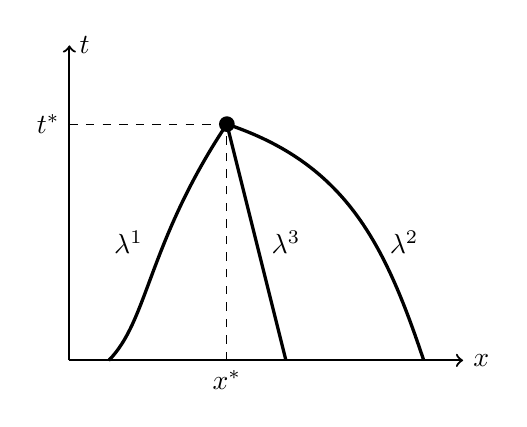
\begin{tikzpicture}
  \draw[thick,->](0,0)--(5,0) node [right] {$x$};
  \draw[thick,->](0,0)--(0,4) node [right] {$t$};
  \fill[black] (2,3) circle (0.1);
  \draw[dashed]  (0,3) node [left] {$t^*$}-- (2,3);
  \draw[dashed]  (2,0)node [below] {$x^*$} -- (2,3) ;
  \draw[very thick] (0.5,0) .. controls (1.,0.5)and (1,1.5) .. (2.,3);
  \draw[very thick] (4.5,0) .. controls (4.,1.5) and (3.5,2.5) .. (2.,3);
  \draw[very thick] (2.75,0) -- (2.,3);
  \node at (0.75,1.5) {$\lambda^1$};
  \node at (2.75,1.5) {$\lambda^3$};
  \node at (4.25,1.5) {$\lambda^2$};
\end{tikzpicture}
%%% Local Variables:
%%% mode: latex
%%% TeX-master: "../../mainManuscript"
%%% End:
